% !TEX root = ../main.tex

% 中英标题:\chapter{中文标题}[英文标题]
\chapter{无人机网络紧急救援模拟系统}[UAV emergency rescue simulation system]

\section{无人机网络紧急救援模拟系统的需求分析}[demand analysis]

\subsection{任务目标}[en title]
无人机网络紧急救援模拟系统是整个无人机救援调度系统的重要组成部分,可以将其视为系统的前端部分。该系统
可以帮助基地中的管理人员更好地了解无人机的实际调度情况和任务分配情况,模拟无人机的物资投放过程。
\subsection{需求详解}[en title]
本系统主要需要实现的功能有待救援地点参数的设置、无人机参数的设置、区域地图显示、前后端功能交互等。
\begin{itemize}
	\item [(1)] 待救援地点参数的设置


    \qquad 用户可以在页面中手动添加待救援点的编号、时间敏感性、位置和名称等信息,也可以通过规格化的数据文件批量导入地点信息;
    \item [(2)] 无人机参数的设置
    

    \qquad 无人机的参数主要指的是在该区域内同时工作的无人机的数量、无人机的型号、载重和续航里程等信息;
    \item [(3)] 区域地图显示
    

    \qquad 用户选择待救援区域的大致范围后,页面将会显示该区域的实际地图,同时无人机、待救援点等地图要素同样会在地图上显示;

    \item [(4)] 前后端功能交互
    

    \qquad 在用户手动输入或批量导入参数信息后,通过页面中的“提交”按钮,前端将地图信息和各种参数传输至后端服务器,由服务器计算
    最优的无人机扫描覆盖路径,再将其传输至前端以供展示最终结果。
\end{itemize}
\section{无人机网络紧急救援模拟系统的设计概要}[design brief]
\subsection{系统框架}[en title]
该系统基于Web设计,使用B/S设计模式,其特点是客户端与服务端分离,通过通信协议进行数据传输,两者内部的实现是独立的,能够降低开发难度和维护难度。前端界面运行于用户浏览器中,使用HTML、CSS和JavaScript实现,并使用Ajax向后端发送和接收数据信息。后端使用Flask框架设计,负责路径规划的计算以及其他后台服务。
本系统中用户只需要选择区域,设置好相关参数,即可开始使用所有的功能。


本系统的设计框架如\figref{fg601}所示:

\begin{figure}[ht]
	\centering
	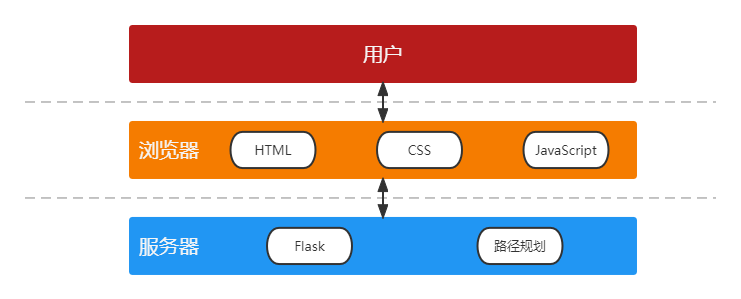
\includegraphics[width = 0.9\textwidth]{fg5_bs}
	\caption{系统设计框架图}
	\label{fg601}
\end{figure}


使用这样的系统框架,可以使得前端界面的展示与后台的路径规划计算相互独立,可以实现高内聚低耦合,降低了今后对于系统的维护成本,实现了前后端分离,提高了工作效率,使得前后端分工更加明确,也能够实现页面的按需加载,可以提高页面交互性能和用户使用体验。

\section{无人机网络紧急救援模拟系统的成果展示}[en title]
\subsection{使用方法}[en title]
在使用本系统时,用户需要在浏览器中打开本系统的网址。页面左侧的是参数设置模块,右侧是实际区域的地图,用户可以根据需要设置待救援点的位置,无人机基地的位置,无人机的数量、型号、载重和续航里程等信息,确认无误后点击“提交”按钮,即可生成最终的规划路径。
\subsection{页面展示}[en title]
如\figref{fg602}所示,系统界面主要分为2个部分,左侧为相关参数的输入设置,右侧为地图的展示区域。地图中除了实际的地图显示,还使用符号标记了用户设置的兴趣点和无人机基地信息。

\begin{figure}[H]
	\centering
	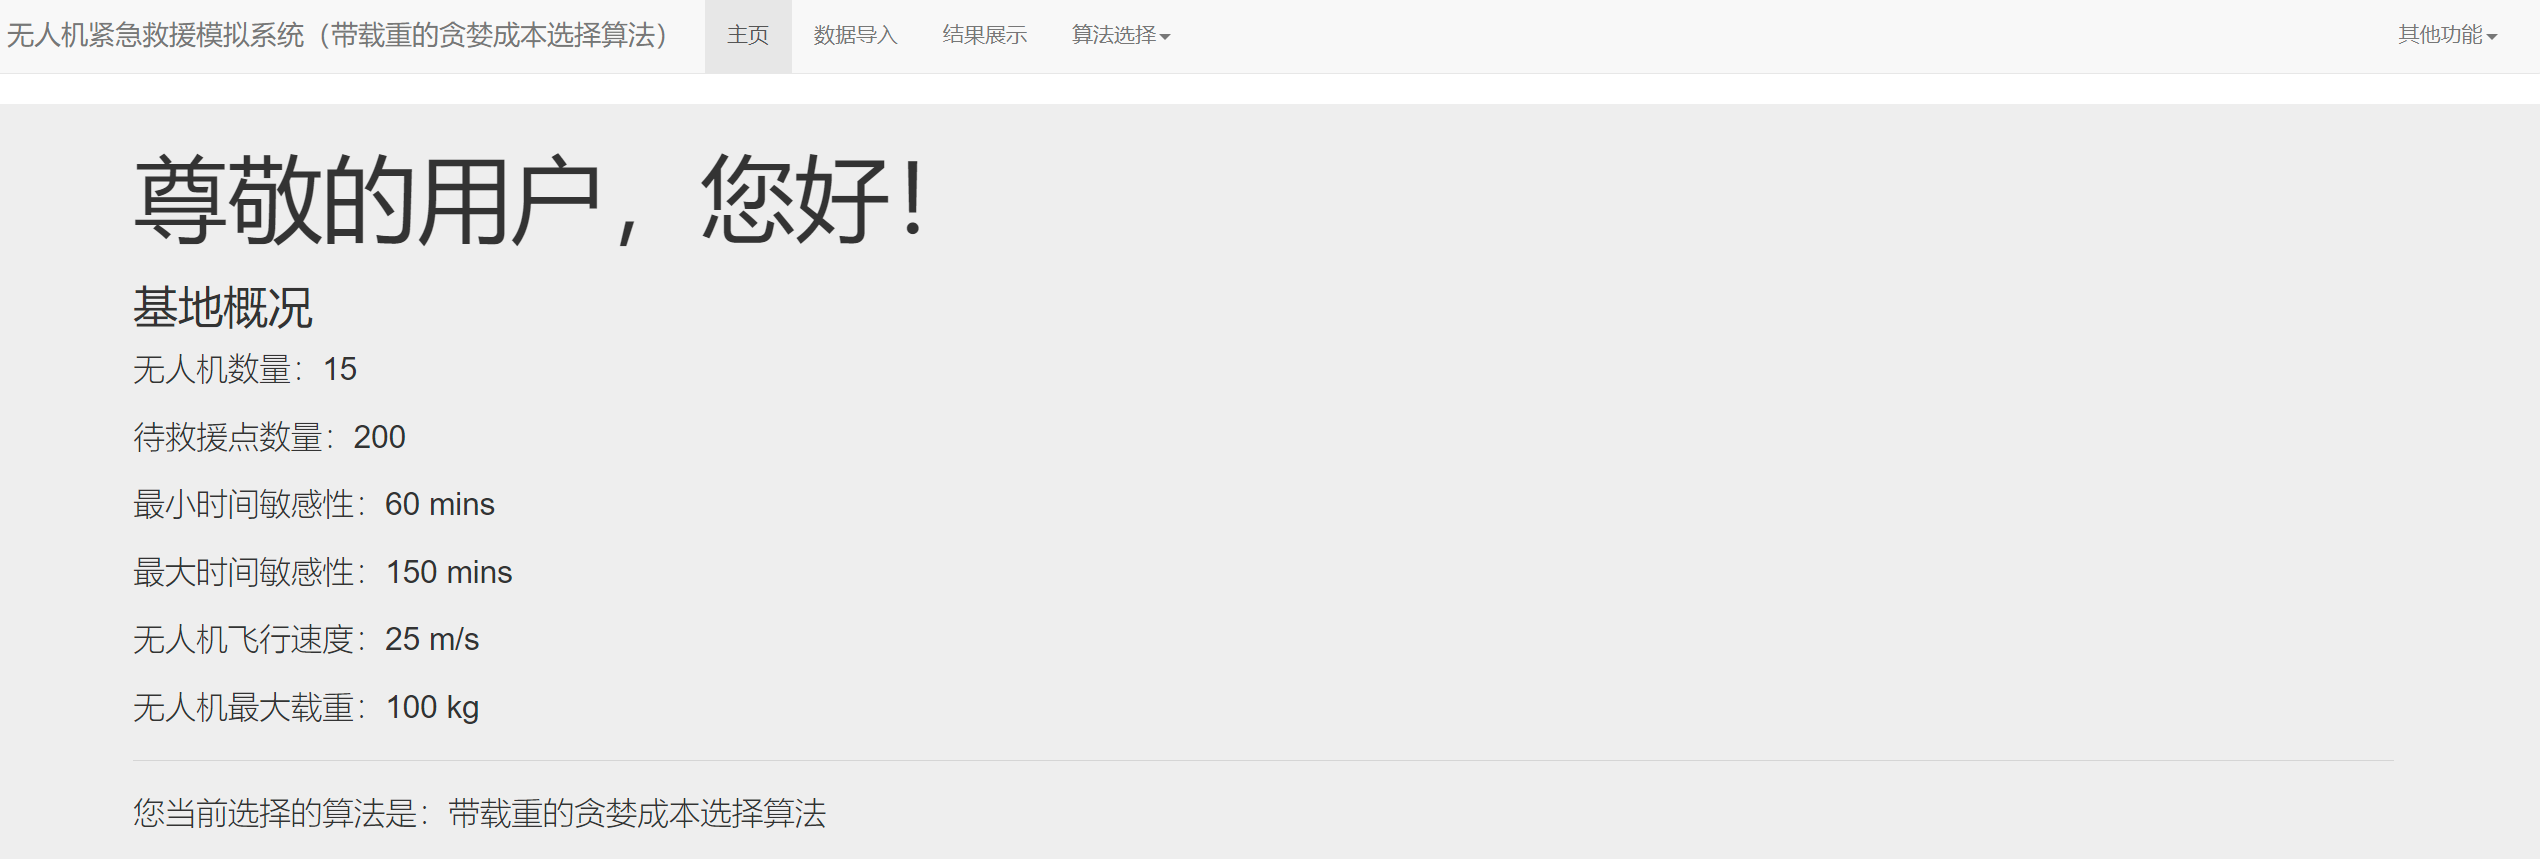
\includegraphics[width = 0.9\textwidth]{fg7_zhujiemian}
	\caption{系统主界面}
	\label{fg602}
\end{figure}
而左侧的参数设置区域又可以分为兴趣点参数设置和无人机参数设置两个模块,分别如\figref{fg603}和\figref{fg604}所示:

\begin{figure}[H]
	\centering
	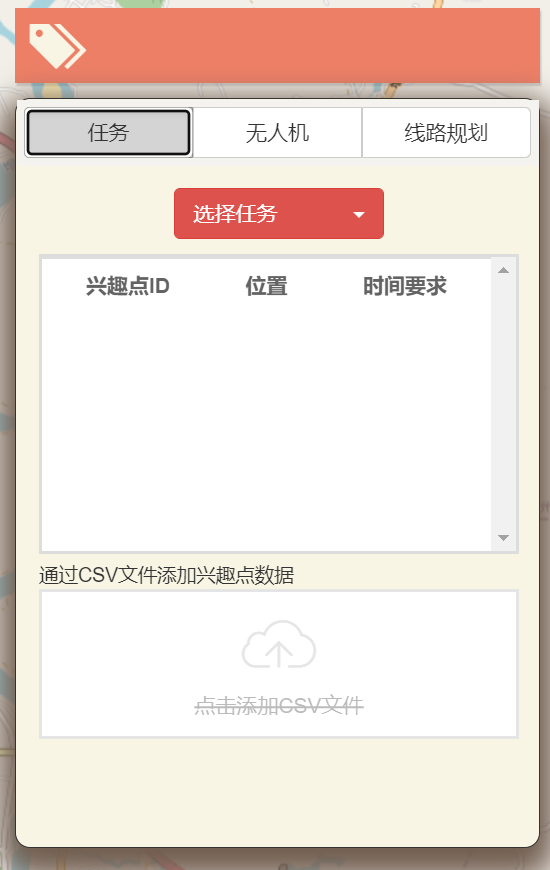
\includegraphics[width = 0.4\textwidth]{fg8_poi}
	\caption{兴趣点参数设置界面}
	\label{fg603}
\end{figure}
\begin{figure}[H]
	\centering
	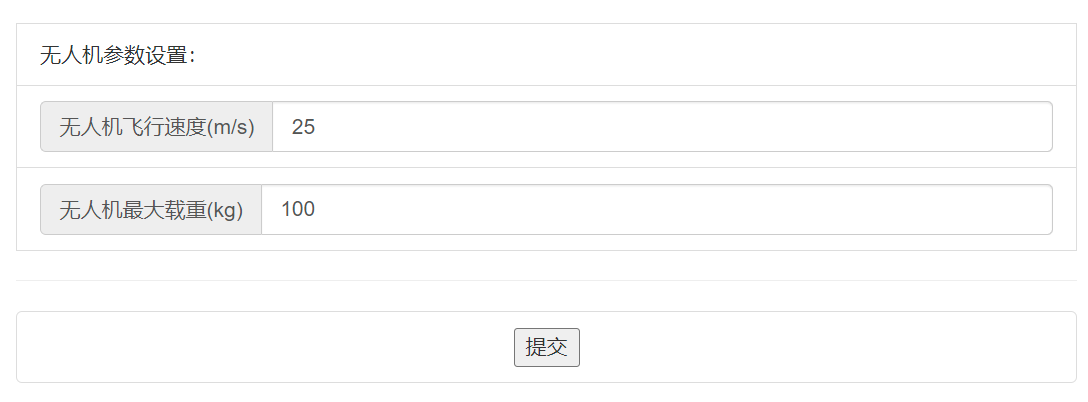
\includegraphics[width = 0.35\textwidth]{fg9_uav}
	\caption{无人机参数设置界面}
	\label{fg604}
\end{figure}
当用户选择了无人机的救援区域并完成了相关的参数设置后,并选择了路径规划所使用的算法后,点击“提交”按钮,前端界面将会把参数和信息通过JSON格式传输至后端,交由其计算最优的无人机飞行路径,再将其传至前端,
这时前端界面便会开始展示无人机的飞行路径。以选择带自交的遗传算法为例,系统页面展示的结果如\figref{fg605}所示:
\begin{figure}[H]
	\centering
	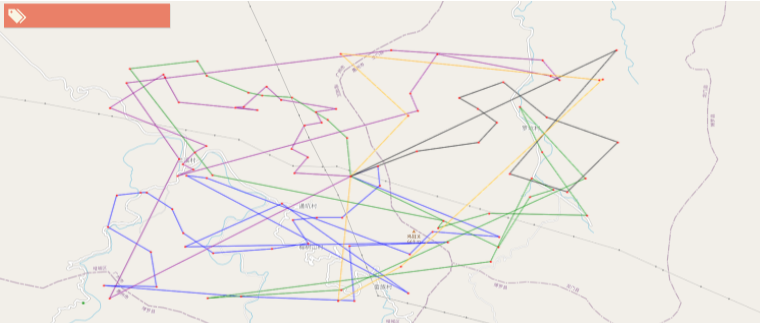
\includegraphics[width = 0.85\textwidth]{fg10_result}
	\caption{在系统中选择带自交的遗传算法后的无人机路径规划结果}
	\label{fg605}
\end{figure}
\section{本章小结}[Brief summary]
本章对无人机网络紧急救援模拟系统进行了设计与实现,并展示了最终的实现效果。